\hypertarget{a-capability-assurance-framework-for-ioc-divestments}{%
\chapter{A Capability Assurance Framework for IOC
Divestments}\label{a-capability-assurance-framework-for-ioc-divestments}}

\hypertarget{from-explanation-to-design}{%
\section{From Explanation to Design}\label{from-explanation-to-design}}

The empirical analysis answered a question of explanation: why broadly
comparable upstream assets, transferred under the same sectoral regime,
produced operators that held operational integrity and operators that
did not. The explanation most consistent with the differentiated
outcomes was capability-related: the operating capability each acquirer
brought, retained, or contracted (Section 4.7). The operators that
failed had not secured the domain-specific upstream operating knowledge
their assets required, and the transaction that transferred the hardware
did not transfer that knowledge with it. The question now becomes one of
design: what transaction and institutional arrangement would make the
capability an asset needs observable before the asset changes hands,
testable against the particular asset, and enforceable afterward? Such a
design would also protect the value placed at risk when operating
capability does not survive the transfer.

The governing idea is a re-specification of an existing rule, not a new
regime. NUPRC's 2024 reforms already require an acquirer to demonstrate
technical capacity, but they assess it primarily at the corporate level,
and corporate-level capacity can pass without any demonstration that the
buyer can run and protect the specific asset it is acquiring. That
variable is re-specified here as asset-specific operating capability,
with the seller disclosure, the structured transfer, and the
post-transfer verification the existing rules leave out added to it, and
each obligation grounded in a hook the law already contains. The aim is
to extend the direction NUPRC has already set, not to work against it.

Why the intervention must be mandatory rather than left to the
transacting parties is a matter of where the value sits. Most of what a
producing asset is worth to the people around it is borne by parties
outside the sale, which is why a price agreed between a willing seller
and a willing buyer underprotects it. Those dimensions, in order of how
far each falls outside the transaction, are set out in Table 5.1.

\begin{longtable}[]{@{}
  >{\RaggedRight\arraybackslash}p{(\columnwidth - 6\tabcolsep) * \real{0.2500}}
  >{\RaggedRight\arraybackslash}p{(\columnwidth - 6\tabcolsep) * \real{0.2500}}
  >{\RaggedRight\arraybackslash}p{(\columnwidth - 6\tabcolsep) * \real{0.2500}}
  >{\RaggedRight\arraybackslash}p{(\columnwidth - 6\tabcolsep) * \real{0.2500}}@{}}
\caption[The value dimensions an operating-capability gap puts at risk]{What operating-capability gaps put at risk: the value dimensions of a divested asset. The two dimensions measured in the empirical analysis begin inside the operator's commercial case and are priced into the sale; operational integrity is the hinge, since its catastrophic failure externalizes costs onto the third parties and the state listed below. The remaining dimensions are borne mostly outside the transaction, which is why a voluntary sale underprotects them and why mandatory verification is warranted. The status column marks which dimensions were demonstrated in the empirical analysis and which are warranted under the framework.}\\
\toprule\noalign{}
\begin{minipage}[b]{\linewidth}\RaggedRight
\end{minipage} & \begin{minipage}[b]{\linewidth}\RaggedRight
Value dimension
\end{minipage} & \begin{minipage}[b]{\linewidth}\RaggedRight
Borne by (incidence)
\end{minipage} & \begin{minipage}[b]{\linewidth}\RaggedRight
Status
\end{minipage} \\
\midrule\noalign{}
\endfirsthead
\toprule\noalign{}
\begin{minipage}[b]{\linewidth}\RaggedRight
\end{minipage} & \begin{minipage}[b]{\linewidth}\RaggedRight
Value dimension
\end{minipage} & \begin{minipage}[b]{\linewidth}\RaggedRight
Borne by (incidence)
\end{minipage} & \begin{minipage}[b]{\linewidth}\RaggedRight
Status
\end{minipage} \\
\midrule\noalign{}
\endhead
\bottomrule\noalign{}
\endlastfoot
& \emph{Internalized by the operator, and priced by the market} & & \\
V1 & Production performance & The operator, with a fiscal and national
shadow & Demonstrated (DV1) \\
V2 & Operational integrity and reliability & The operator while running;
third parties on catastrophic failure & Demonstrated (DV2) \\
& \emph{Externalized, borne by others} & & \\
V3 & Safety and environmental harm to third parties & Workers,
contractors, communities, ecosystems, the state's remediation liability
& Warranted \\
V4 & Host-community welfare & Host communities & Warranted \\
V5 & National capability development & The Nigerian workforce and
economy & Warranted \\
V6 & Fiscal and public-revenue protection & The state & Warranted \\
V7 & Energy security and production resilience & The nation & Warranted,
with the theft, sabotage, and price confound \\
V8 & Decommissioning and abandonment responsibility & The state and
future generations & Warranted, with a financial-security mandate \\
\end{longtable}

The hinge is in the second row. The upkeep of operational integrity is
internalized, so an operator captures the savings from deferring it, but
the catastrophic failure that deferral invites is externalized onto the
dimensions below. The transaction market therefore does not reliably
correct the problem on its own, and verification cannot be left to the
parties. Production capability is protected alongside safety, since the
same operating knowledge carries both; what is verified is readiness,
not a guaranteed level of output.

The dimensions below the hinge fall outside the transaction in distinct
ways, and each names a reason the private bargain underprotects the
public interest. Safety, environmental, and community harm (V3, V4) are
the catastrophic-failure costs the hinge externalizes directly. The
remaining four fall outside the sale for different reasons. National
capability development (V5) is the workforce capacity that the
local-content regime exists to build and that a hollowed-out transfer
sets back. Fiscal protection (V6) is the royalty and tax base that
erodes as production and integrity decline. Energy security (V7) is the
national production resilience that weak operations put at risk, with
theft and price as confounds. Decommissioning (V8) is the abandonment
liability that outlives the operator and falls to the state and future
generations. Each sits further from the sale than the last, and that
distance is the measure of how little an agreed price protects it.

The claim is bounded in two ways. The empirical regularities and the
design logic warrant the framework, short of proof from a tested
intervention, and what it assures is demonstrated capability and
readiness, not a guaranteed outcome. It is also calibrated to a
particular setting. That setting has aged Niger Delta assets carrying
integrity backlogs and suspended wells, a security and theft environment
that raises the cost of weak operations, and a community and
public-revenue structure that bears the failures the transacting parties
do not. It works within an existing architecture of NUPRC regulations,
the Nigerian Oil and Gas Industry Content Development Act (NOGICD), and
the Petroleum Industry Act (PIA) that the framework works through rather
than replaces. A design built for these conditions would need re-fitting
for others.

What follows is a warranted design, not a costed implementation plan and
not a claim that any single design guarantees success. What operating
capability is, and why it does not reconstitute on its own, comes first
(Section 5.2), followed by why the market and the existing rules do not
deliver it (Section 5.3). The framework itself, three mutually
constraining roles across the transaction lifecycle, is set out next
(Section 5.4), then calibrated against Nigerian and comparator
international practice (Section 5.5) and scaled to the risk a given
transaction carries (Section 5.6). Finally, the jurisdictional and
operational limits of the warrant are established (Section 5.7).

\hypertarget{the-embedded-nature-of-operating-capability}{%
\section{The Embedded Nature of Operating
Capability}\label{the-embedded-nature-of-operating-capability}}

The relevant capability is not generic managerial competence. It is
domain-specific upstream operating knowledge embedded in people,
routines, integrity and emergency systems, decision rights, and data,
and when its carriers are not retained, the gap can surface as a safety
failure. A divestment moves the license, the wells, the platforms, and
the pipelines. It does not, on its own, move the knowledge of how that
particular asset is run safely and productively, because most of that
knowledge lives in the people who operate it and in the routines,
records, and relationships they have built around it over years.

That capability, defined in Section 2.2, can be described as a bundle of
six families. The first is the operating workforce itself, the
engineers, controllers, and supervisors who hold the tacit feel for how
the asset behaves and what it tolerates (Kogut and Zander, 1992). The
second is the body of operating routines, the procedures and practices
that translate general engineering standards into the specific handling
of this reservoir, this terminal, this set of aging wells. The third is
the integrity and emergency systems, the inspection histories, the
maintenance backlogs, the contingency plans, and the standing
arrangements to respond when something fails. The fourth is the
structure of decision rights and accountability, the question of who is
authorized to act, and how fast, when a well begins to lose control. The
fifth is the asset's data and history, the record of what has been done,
deferred, and discovered across decades of operation. The sixth is the
contractor and technical-support architecture, the web of specialist
firms a competent operator keeps on call before a crisis rather than
after one. Taken together, these six families are the architecture of
the operating enterprise, the organization, routines, knowledge,
decision rights, data, and external relationships through which the
physical assets are made to produce safely. Enterprise architecting
treats this organizational architecture, not the physical plant alone,
as the enterprise (Nightingale and Rhodes, 2015), so a divestment that
conveys the plant without it transfers the hardware without the system
that runs it.

These families map the same ground that the process-safety literature
organizes, at finer grain, into an established set of elements. The
Center for Chemical Process Safety organizes operating capability into
twenty elements across four pillars, under the heading of Risk-Based
Process Safety, or RBPS (CCPS, 2007). The four pillars are a commitment
to safety, an understanding of hazards and risk, the management of that
risk in daily operation, and the discipline of learning from experience.
That four-pillar structure is the backbone for operating integrity in
the analysis that follows, chosen because it is independent of any
single operator, widely used across the industry, and auditable. It was
also chosen because mapping each obligation onto a recognized element
keeps the design traceable rather than ad hoc. The condensed bundle
appears as Table 5.3 (Section 5.4); the full element-by-element trace,
from each RBPS element to Ferreira's transfer factors, the empirical
evidence, the legal hooks, and the value dimensions, is in Appendix G.

Risk-Based Process Safety carries the integrity side of performance. It
does not, by itself, capture production. Production performance and
operational integrity are the two dimensions of value at risk in the
cases examined (Sections 4.5 to 4.7). The capability that sustains
output, the subsurface understanding and the production-operations
discipline that keep a field flowing, is as embedded and as perishable
as the capability that keeps it safe. A production and subsurface
operating-capability element therefore sits alongside the four
process-safety pillars and on the same footing, not beneath them.
Production performance is monitored as a value dimension and linked to
that subsurface and production-operations capability; what is verified
is readiness, not guaranteed output.

If the four pillars and the production element describe what capability
is, a separate body of work describes what becomes of it during a
handover. Ferreira et al.~(2024) study the transfer of knowledge between
operators during the sale of an aging offshore asset and identify
twenty-two elements that determine whether knowledge actually moves from
seller to buyer. The elements range from the structure of the contract
and the availability of the seller's professionals to the access the
buyer is granted to databases and the time allowed for the transfer to
happen. They are not the capability itself but the conditions under
which it transfers or is lost, and they depend as much on the buyer's
capacity to receive and absorb knowledge as on the seller's willingness
to release it (Cohen and Levinthal, 1990).

The link between the two, between a failed transfer condition and a
degraded operating element, has been traced directly. In a content
analysis of the same transfer, Ferreira et al.~(2026) map these transfer
conditions onto the process-safety elements each degrades when it fails,
and report that process-safety incidents rose, in both frequency and
severity, after an aging asset changed hands without retention of its
operating team. That content analysis directly codes ten of the twenty
process-safety elements; in Appendix G the mapping is extended to the
remaining ten from the cases and the legal hooks, with the directly
coded links flagged as coded and the inferred ones as inferred. The path
is concrete. When the contract is silent on operational requirements,
the elements that suffer are emergency management, asset integrity, and
hazard analysis. When the transfer period is compressed and records
arrive piecemeal, the management of process knowledge erodes first, and
it is the element on which the largest number of these transfer failures
converge. When the people and records that hold operating knowledge are
not retained, the gap can stay latent for a time, but the evidence shows
it tends to surface as higher incident frequency and severity.

The six cases divide on exactly this point. The operators that sustained
both output and integrity had absorbed the capability rather than merely
acquired the assets. Seplat brought an experienced upstream organization
under Austin Avuru and operated in partnership with Maurel et Prom;
HEOSL operated OML 30 through Salvic as its technical operator,
retaining the operating competence the license assumed (Sections 4.5.1
and 4.5.2). Neither rebuilt that capability after the fact; each had it
in place at transfer or held it through the operator it brought. The
operators whose performance diverged had taken on the hardware without
the embedded system that made it work. Aiteo, whose founder and chief
executive came from a downstream trading background, inherited the wells
of OML 29 without the well-control capability they demanded. The Santa
Barbara blowout of November 2021 is where that absence became visible:
no contingency plan, no standing well-control contract, and a specialist
response contractor engaged only once the well was already flowing
uncontrolled (Sections 4.3.1 and 4.3.6). The license transfer moved the
asset; what it did not do was make the missing well-control capability
visible, testable, or enforceable before close.

Operating capability, then, is embedded, perishable, and specific to the
asset, and in the cases examined it did not reconstitute itself in the
hands of a new owner within operationally relevant timeframes. Whether
it survives a sale depends on conditions that are observable at the
point of transfer, what the seller discloses, what the buyer can absorb,
and what the regulator verifies, and on whether the buyer is built to
receive what is offered. Nigeria's 2024 divestment framework now creates
a technical-capacity route at consent. Whether that route reaches what
this asset needed, asset-specific crisis readiness, a structured
transfer, demonstrated buyer absorption, and verification after close,
is the open question.

\hypertarget{the-market-and-regulatory-failure-to-transfer-capability}{%
\section{The Market and Regulatory Failure to Transfer
Capability}\label{the-market-and-regulatory-failure-to-transfer-capability}}

In the case analysis, the embedded operating capability a buyer
inherited, brought, or contracted before performance depended on it,
rather than capital constraints or fiscal terms alone, best separated
the operators that sustained performance from those that did not
(Sections 4.5 and 4.7). If that capability is what a divested asset
needs, why does a buyer not reliably acquire it, and why does the
consent regime that governs the transfer not require it? The transaction
structure makes that loss structurally likely rather than accidental,
through four gaps that compound across the seller, the buyer, and the
parties outside the deal. And the rules that gate the transfer measure
corporate and compliance attributes instead of demonstrated operating
capability, and confirm nothing once the asset has changed hands.

\hypertarget{the-pre-transfer-condition-and-disclosure-gap}{%
\subsection{The Pre-Transfer Condition and Disclosure
Gap}\label{the-pre-transfer-condition-and-disclosure-gap}}

Operating capability is not a static inventory. Its tacit component
erodes when it is not exercised, and the record of an asset's embedded
requirements, its integrity history, and its near-misses lives partly in
documents and partly in the people who ran it (Kogut and Zander, 1992;
Nonaka, 1994). A seller preparing to exit holds that record, and has
incentives to limit transition exposure, protect proprietary operating
knowledge, and avoid new spending whose benefit would accrue mainly
after close. What was never written down cannot be recovered from a data
room.

The evidence is the condition of what Aiteo inherited: a well at Santa
Barbara that was suspended and undecommissioned at transfer. The
reviewed record does not show that the well's condition became an
approval condition, a readiness test, or a verified handover obligation
(Section 4.3.1). The corpus contains no admission by a seller that it
cut spending before a sale, and none is needed. The provable claim is
narrower: the information needed to assess what is being inherited sits
with the seller, and the reviewed rules do not yet compel its disclosure
in asset-specific, verifiable form. Nigeria's content law requires a
Nigerian Content Plan and Certificate of Authorization before
acquisition (NOGICD Sections 7-9), and the NUPRC divestment guidance
calls for a facility catalog and asset register. A catalog lists what
exists, not its condition or the operating knowledge the asset demands.
Neither obliges the seller to disclose asset condition, integrity and
incident history, and embedded operating requirements in a form a buyer
and a regulator could use to judge the inheritance.

\hypertarget{information-asymmetry-and-adverse-selection}{%
\subsection{Information Asymmetry and Adverse
Selection}\label{information-asymmetry-and-adverse-selection}}

The condition gap becomes an economic problem once the seller's
incentives are added. The seller knows the embedded difficulty of the
asset, the buyer does not, and disclosure of that difficulty lowers the
price. The better-informed party therefore gains from limiting what
becomes price-relevant. This is the adverse-selection structure
developed earlier from Akerlof (1970): where quality is hidden and the
informed side has reason not to reveal it, the market does not price it
correctly, and the uninformed side overpays for what it cannot verify.
Tacit operating knowledge is the hardest case, because it is not fully
contractible even when the seller is willing. It cannot be reduced to a
schedule and warranted.

The asymmetry is visible directly in the cases. The seller knew the
asset's operating requirements, the buyer could not assess them from the
data room, and the regulator lacked the tools to close the gap on either
side (Section 4.3.3). The existing consent gate turns on ministerial
approval and a technical-capacity test conducted mainly at the corporate
level (PIA Section 95; NUPRC Reg. 7), with asset-specific demonstration
and site inspection not mandatory in every case; neither obtains
standardized disclosure from the seller nor independently verifies
demonstrated operating capability in the buyer. The asymmetry is
therefore left to voluntary seller disclosure, by the party with the
least reason to volunteer.

\hypertarget{the-buyers-absorptive-capacity}{%
\subsection{The Buyer's Absorptive
Capacity}\label{the-buyers-absorptive-capacity}}

Even full disclosure and a willing seller do not transfer capability if
the buyer cannot receive it. Absorptive capacity, a firm's ability to
recognize the value of external knowledge, assimilate it, and apply it,
is itself a function of prior related expertise (Cohen and Levinthal,
1990). A buyer without upstream operating depth lacks the foundation
needed to receive and integrate what is transferred. This is a
buyer-side constraint rather than a seller incentive, and the market
cannot supply it on demand.

The contrast across the cases is sharp. Seplat, built on a founding team
of upstream operators and reinforced by Maurel et Prom, and the OML 30
operator, staffed through Salvic, retained or brought equivalent
operating people and absorbed what they inherited. Aiteo, led from a
downstream trading background, did not (Sections 4.5.1 and 4.5.2). The
transfer-process evidence points the same way: incidents rose in
frequency and severity after handover where the operating team was not
retained and the transfer terms did not secure continued access to the
people and data that held the asset's knowledge (Ferreira et al., 2026).
Nigeria's content law holds the nearest statutory analogue, a four-year
understudy succession and technology-transfer provisions (NOGICD Section
31; Sections 43-47). It was written to localize a single operator's
workforce over time, not to guarantee that a new operator can absorb an
asset at the point of handover.

\hypertarget{the-externality}{%
\subsection{The Externality}\label{the-externality}}

The first three gaps explain why a buyer may end up without the
capability an asset needs. The fourth explains why the public, and not
the contracting parties, must be the one to act. When operating
capability fails, the largest costs do not fall on the buyer or the
seller. They fall on the communities exposed to a spill or a blowout, on
the state that loses production and revenue, and on a future public that
will bear the abandonment liability. Welfare economics has named this
divergence since Pigou: where private actions impose costs on third
parties that market prices do not reflect, the private optimum sits
below the social optimum, and correction calls for public intervention
rather than private goodwill (Pigou, 1920).

The obvious objection is Coase. If the affected parties could bargain
with the transacting parties, they would reach an efficient outcome
without a regulator, whatever the initial allocation of rights (Coase,
1960). That route is closed here. The parties who bear the cost of a
capability failure run to tens of communities and extend to a general
and future public that cannot be assembled at the table before consent
is granted. Transaction costs are prohibitive, the Coasean solution is
unavailable, and the Pigouvian case for mandatory public verification
stands. The empirical analysis documented the more direct externalities:
the 41 communities affected by the Santa Barbara blowout and the seven
deaths in the separate Benin River explosion. The national production
shortfall, near 1.5 against a target of roughly 2 million barrels per
day, provides sector-level context rather than a case-specific causal
estimate, since theft, sabotage, investment cycles, and price conditions
also bear on it (Section 4.7.3). Nigeria already addresses parts of this
externality after the fact, through Host Community Development Trusts
and a decommissioning fund, and the 2024 framework secured more than
US\$400 million in decommissioning escrow (PIA Chapter 3; Sections
232-233; NUPRC pillars 4 and 5). Those mechanisms compensate for harm or
fund eventual abandonment. None of them verifies the operating
capability that would prevent the harm in the first place.

The four gaps are set out together in Table 5.2, with the evidence for
each and the requirement each implies.

\begin{longtable}[]{@{}
  >{\RaggedRight\arraybackslash}p{(\columnwidth - 6\tabcolsep) * \real{0.2500}}
  >{\RaggedRight\arraybackslash}p{(\columnwidth - 6\tabcolsep) * \real{0.2500}}
  >{\RaggedRight\arraybackslash}p{(\columnwidth - 6\tabcolsep) * \real{0.2500}}
  >{\RaggedRight\arraybackslash}p{(\columnwidth - 6\tabcolsep) * \real{0.2500}}@{}}
\caption[The four structural gaps behind an unassisted-divestment capability gap]{The four structural gaps that make an operating-capability gap the likely outcome of an unassisted divestment. The gaps compound, from the asset condition and capability the seller does not disclose, through a buyer that may be unable to absorb what is transferred, to the failure costs that fall on parties outside the transaction, which is why correction cannot be left to the contracting parties. In each row, the existing consent rules verify a corporate or compliance attribute, short of the demonstrated operating capability the gap concerns.}\\
\toprule\noalign{}
\begin{minipage}[b]{\linewidth}\RaggedRight
The gap
\end{minipage} & \begin{minipage}[b]{\linewidth}\RaggedRight
Evidence (Chapter 4)
\end{minipage} & \begin{minipage}[b]{\linewidth}\RaggedRight
What the current rules verify
\end{minipage} & \begin{minipage}[b]{\linewidth}\RaggedRight
What the framework requires
\end{minipage} \\
\midrule\noalign{}
\endfirsthead
\toprule\noalign{}
\begin{minipage}[b]{\linewidth}\RaggedRight
The gap
\end{minipage} & \begin{minipage}[b]{\linewidth}\RaggedRight
Evidence (Chapter 4)
\end{minipage} & \begin{minipage}[b]{\linewidth}\RaggedRight
What the current rules verify
\end{minipage} & \begin{minipage}[b]{\linewidth}\RaggedRight
What the framework requires
\end{minipage} \\
\midrule\noalign{}
\endhead
\bottomrule\noalign{}
\endlastfoot
\textbf{1. Condition and disclosure.} Tacit knowledge erodes when
unexercised; the seller holds the asset's condition and operating record
(Kogut and Zander, 1992; Nonaka, 1994). & Aiteo inherited a suspended,
undecommissioned well at Santa Barbara (Section 4.3.1). & A Nigerian
Content Plan and a facility catalog: what exists, not its condition
(NOGICD Sections 7-9; NUPRC guidance). & The seller discloses asset
condition, integrity and incident history, and embedded operating
requirements. \\
\textbf{2. Adverse selection.} The seller knows the embedded difficulty,
the buyer cannot, and disclosure lowers the price (Akerlof, 1970). & The
buyer could not assess operating requirements from the data room, and
the regulator lacked the tools (Section 4.3.3). & Ministerial consent
and a technical-capacity test conducted mainly at the corporate level
(PIA Section 95; NUPRC Reg. 7). & Standardized disclosure and
independent verification of demonstrated operating capability. \\
\textbf{3. Absorptive capacity.} A buyer without upstream depth cannot
receive and integrate transferred knowledge (Cohen and Levinthal, 1990).
& Seplat and the OML 30 operator absorbed; Aiteo, downstream-led, did
not; incidents rose where teams were not retained (Sections 4.5.1-4.5.2;
Ferreira et al., 2026). & A four-year understudy written for one
operator over time, not for a handover (NOGICD Section 31; Sections
43-47). & The buyer demonstrates absorptive capacity; a technical
operator or understudy and a team-retention plan for de novo buyers. \\
\textbf{4. Externality.} The cost of a capability failure falls on third
parties who cannot bargain before consent (Pigou, 1920; Coase, 1960). &
41 communities affected at Santa Barbara; seven deaths at Benin River;
sector-level production shortfall (Section 4.7.3). & Host-community
trusts and a decommissioning fund: compensation and abandonment cover
after the fact (PIA Chapter 3; Sections 232-233). & Public, enforceable
verification; financial security tied to decommissioning; community
standing. \\
\end{longtable}

\hypertarget{the-wrong-variable-diagnosis}{%
\subsection{The Wrong-Variable
Diagnosis}\label{the-wrong-variable-diagnosis}}

The four gaps make an operating-capability gap structurally likely in an
unassisted transfer. The natural question is whether the existing
consent regime catches it, and the regime is more thorough than it is
often given credit for. NUPRC's upstream asset divestment framework
assesses seven pillars at consent through the Nigeria Upstream Petroleum
(Assignment of Interest) Regulations 2024, and the content law adds
pre-acquisition participation and succession requirements. The
difficulty is not that the machinery is thin. It is that it measures the
wrong variable.

A single test makes the point. Walk the consent requirements, and after
each one ask whether it obliges the operator to demonstrate that it can
contain a well-control event of the kind that occurred at Santa Barbara.
The seven-pillar technical-capacity assessment evaluates capacity mainly
at the corporate level, with a site visit left to the regulator's
discretion (NUPRC Reg. 7); it does not. The Nigerian Content Plan and
Certificate of Authorization establish local-content participation
(NOGICD Sections 7-9); they do not. The understudy and
technology-transfer provisions localize a workforce over years (NOGICD
Section 31; Sections 43-47); they do not. Ministerial consent is a legal
and fiscal gate (PIA Section 95); it does not. The Host Community
Development Trusts provide for welfare once the asset is operating (PIA
Chapter 3); they do not. The answer is the same down the list. None of
these requirements compels a mandatory, asset-specific demonstration of
crisis readiness before close, or verification after it. The diagnosis
is therefore one of specification and closure, not absence: the
technical-capacity route exists, but it reaches none of the
asset-specific disclosure, transfer, absorption, and verification the
four gaps require.

This is a re-specification, not a condemnation. The rules are
well-intentioned and have grown more demanding, and the 2024 reform,
including the decommissioning escrow, narrows the gap without closing
it. The First Hydrocarbon transfer of OML 26 illustrates the older gap
rather than the current one. It passed under the prior regime to a buyer
whose backers were later convicted of fraud (Section 4.4.2), and the
2024 Regulations have partly closed that particular opening by screening
directors for prior convictions. The point is not that the later fraud
could have been detected at the time of the transfer; it is that buyer
fitness and governance integrity were not structured approval questions
under the earlier framework. What the regime still does not do is
require the operating-capability demonstration that the four gaps make
necessary.

\hypertarget{the-same-gap-across-acquisition-pathways}{%
\subsection{The Same Gap Across Acquisition
Pathways}\label{the-same-gap-across-acquisition-pathways}}

The gap is not peculiar to the bilateral IOC-to-indigenous sale,
although that transaction is the textbook adverse-selection setup. It
recurs wherever Nigeria has allocated operatorship without verifying
operating capability. The marginal field program awarded acreage on
signature bonuses, work-program commitments, and farm-out arrangements,
with no effective operating-capability screen, a structural precedent
for transferring operations to parties whose ability to run them was
never tested (Section 4.6). The state route shows the same pattern. At
NPDC, political standing sustained operatorship and commercial
participation without the operational demonstration a capability test
would require (Section 4.5.3). An NPDC-authored assessment of indigenous
service companies found that table-top scoring passed firms that failed
on facility inspection, with fewer than half meeting the benchmark once
equipment and personnel were examined on site (Oriaku et al., 2016).
Paper capability and demonstrated capability are not the same thing, and
only a site-level test separates them.

Voluntary standards cannot close the gap either. The industry's
process-safety and management-system guidance describes the right
capability content. The guidance is voluntary, internal to a single
operator, blind to the moment of transfer, and dependent on voluntary
adoption by the buyer, including buyers whose capability is the issue in
question, a point developed in Section 5.5.3. An independent
civil-society proposal, the National Principles for Responsible
Petroleum Industry Divestment, is consistent with much of the same
logic. It calls for seller disclosure of liabilities, demonstrated
technical and financial capacity assessed by an independent body, and an
asset-integrity review with deficiencies remedied before approval
(Steiner, 2023). The design set out in the next section is grounded in a
capability theory and the critical-experiment evidence. It goes beyond
those proposals by incorporating the buyer's absorptive capacity and the
structure of the transfer itself, extending assurance past close into
verification, and working through existing statutory hooks in place of a
new voluntary instrument.

The case for intervention follows from these findings together. On its
own, the transaction underprovides capability transfer: the structure
leaves the gap unpriced, the existing rules verify corporate and
compliance attributes and stop at consent, well short of demonstrated
capability, and the cost of failure falls on parties never at the table
(Table 5.2). The institutional design that resolves this, set out in
Section 5.4, makes operating capability something a seller must
disclose, a buyer must demonstrate, and a regulator must verify, before
and after the asset changes hands.

\hypertarget{the-capability-assurance-framework}{%
\section{The Capability Assurance
Framework}\label{the-capability-assurance-framework}}

A specific institutional design follows from that diagnosis.
Corporate-level technical capacity can clear consent without
asset-specific operating capability being disclosed, absorbed, or
verified. The remedy is to re-specify the existing hooks so that those
three things happen, and to connect them, so that none is satisfied on
paper while another is left undone. Three roles carry the design. The
seller discloses, the buyer absorbs, and the regulator verifies, across
the life of the transaction and within the consent, content, and labor
provisions Nigeria already has. Together the three roles form a control
structure, in the systems-theoretic sense of the control actions and
feedback that hold a hazardous process within safe bounds (Leveson,
2011), organized around the asset as a sociotechnical system. The
divestment moves the technical subsystem, the wells and the facilities,
but not the social subsystem that operated it (Section 2.2). The design
exists to make the disclosure, transfer, and verification of that social
subsystem happen across the transaction instead of being left to the
discretion of the transacting parties. It thereby installs the
corrective function the market does not supply, the one severed because
the costs of operational failure fall outside the sale (Section 2.6).
The framework can be built primarily through existing consent,
due-diligence, content, labor, and decommissioning hooks, although some
elements would require regulations, consent conditions, or license
terms.

\hypertarget{three-roles-in-a-closed-loop}{%
\subsection{Three Roles in a Closed
Loop}\label{three-roles-in-a-closed-loop}}

The three roles are not a sequence of independent checks. Each depends
on what the others produce. Disclosure gives the buyer and the regulator
something concrete to work with, the asset's condition and the
operating-capability bundle defined in Section 5.2. Absorption is
meaningful only when it is tested against what was disclosed, so that a
buyer's claim to competence is matched to the specific demands of this
asset instead of asserted in general. Verification constrains both and
rests on both, because the regulator can confirm only what the seller
has surfaced and the buyer has shown. Each role enables and constrains
the others, which is why the design closes into a loop rather than
running down a checklist.

The loop is built around a feature of the documented failures: they were
not isolated to one party. At Aiteo, an inherited undecommissioned well,
the buyer's missing well-control capability, and the regulator's lack of
any tool to test for it were present at the same time (Sections 4.3.1
and 4.3.6). A checklist that cleared each party in isolation would have
passed the transaction, because each gap was not visible, within the
consent process, to the party that might have caught it. A loop checks
each role against what the others produce, so that a gap left open in
one place has somewhere to be caught.

The regulator's role is a verification overlay rather than a party to
the transfer. The transfer-process literature describes a bilateral
exchange between seller and buyer (Ferreira et al., 2024); the third
role rests on a different basis. It draws on the consent and
fit-and-proper powers the regulator already holds (PIA Section 95; NUPRC
Reg. 7), on the externality that places the cost of failure on parties
outside the transaction (Section 5.3.4). It also rests on the practice
of mature petroleum regulators that assess capability by demonstration
rather than declaration, Norway through prequalification before entry
and Alberta through assessment of both transferor and transferee at
transfer (both developed in Section 5.5). The loop is shown in Figure
5.1.

\begin{figure}[H]
\centering
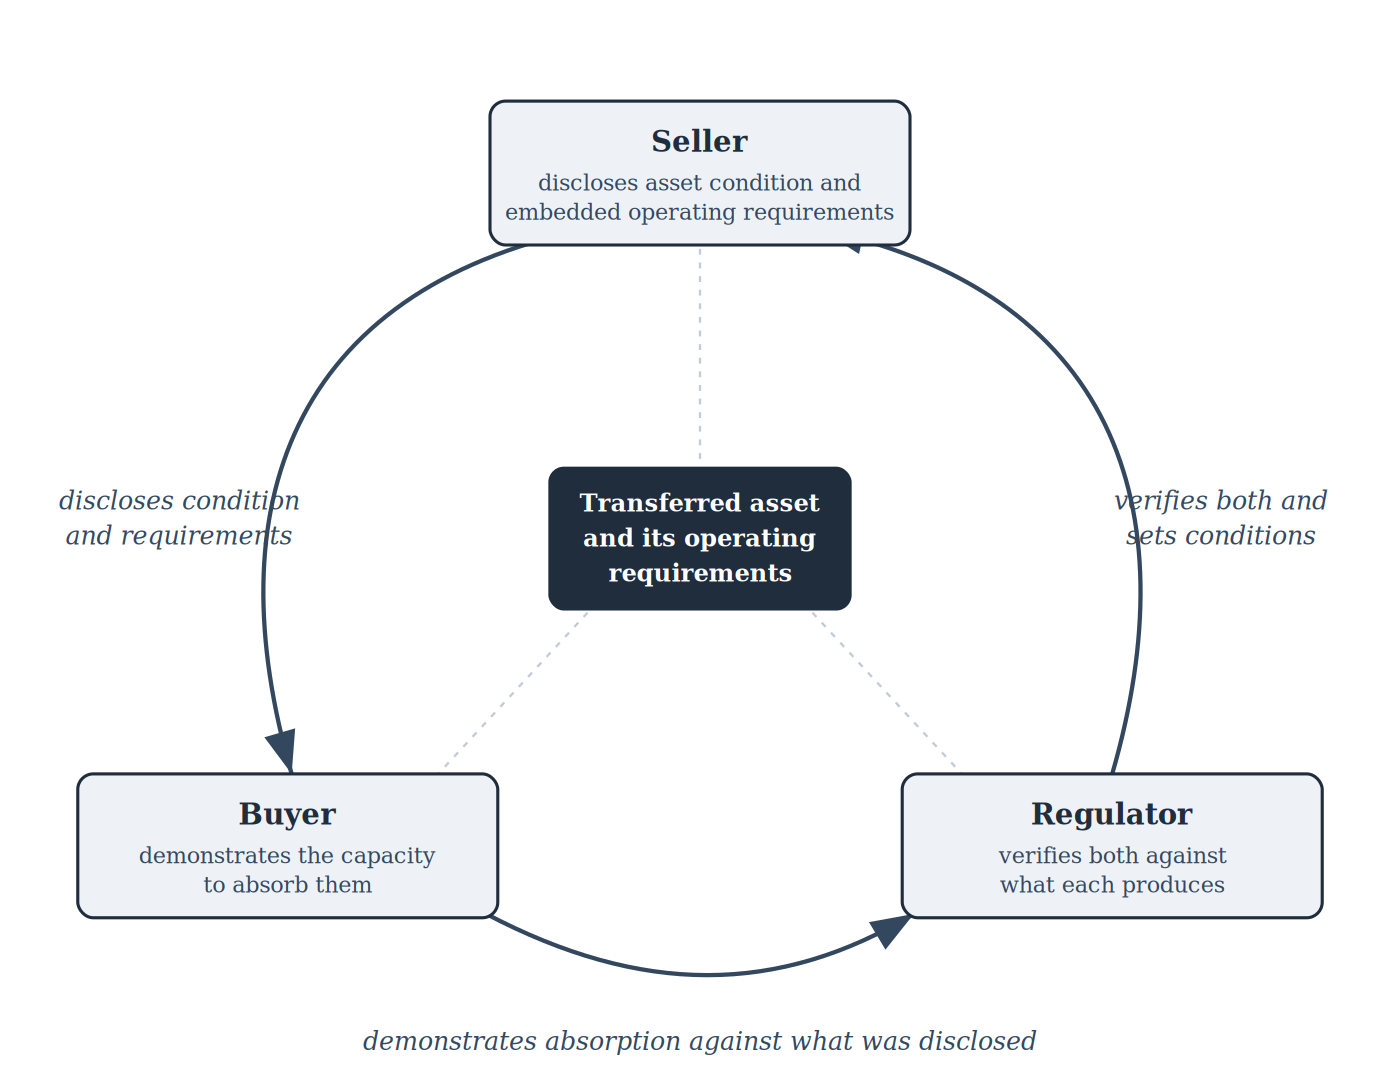
\includegraphics[width=\textwidth,height=0.45\textheight,keepaspectratio]{Figure_5_1_capability_assurance_loop.png}
\caption[The capability assurance loop]{The capability assurance loop. Seller disclosure, buyer absorption, and regulator verification act as three mutually constraining roles around the transferred asset. Weakness in any one role breaks the assurance, because the next role is left with nothing to act on.}
\end{figure}

That is the structure of the loop, which role acts on what. Its dynamics
are the complement: the same three roles are three balancing
interventions on the degrading cycle of Figure 2.1. Mandatory seller
disclosure closes the information gap at the point of sale; buyer
absorption verification confirms the capability before handover; and the
regulator's verification mandate, with rule-based triggers, installs the
requirement and restores the corrective signal the market does not send.
Each intervention cuts a different link, and the degrading cycle is
broken only when all three act together: a single intervention is
unlikely to close it, which is why disclosure without verification, or
verification without a buyer able to absorb, does not hold. Figure 5.2
places the three interventions on the same loop. Across the thesis the
three figures form one sequence: Figure 2.1 sets out the failure
equilibrium, Figure 5.1 the capability assurance loop that would close
it, and Figure 5.2 the points at which the framework cuts that loop.

\begin{figure}[H]
\centering
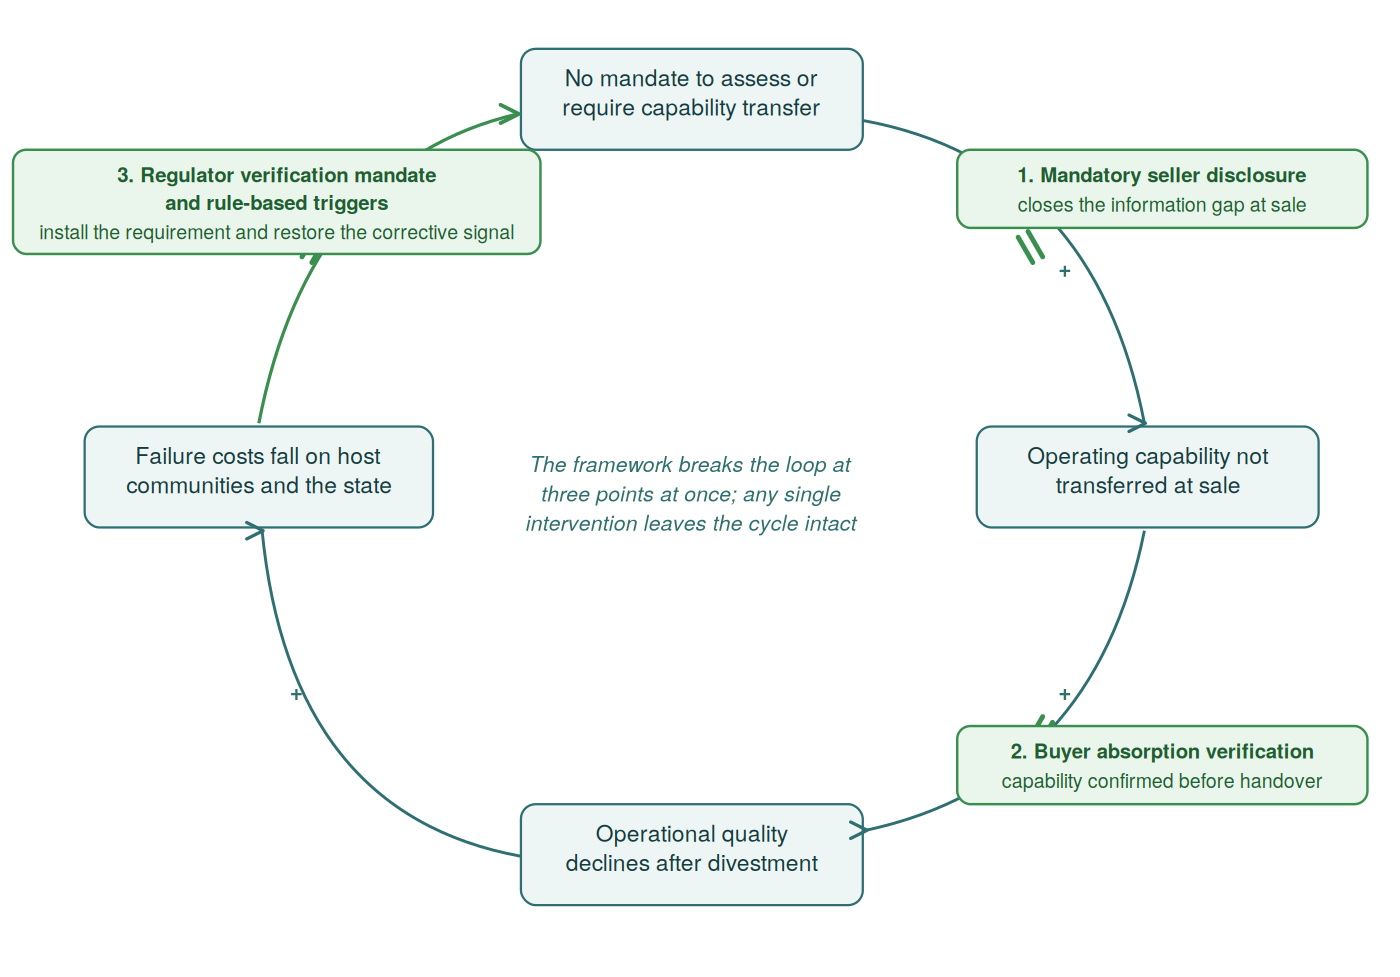
\includegraphics[width=\textwidth,height=0.45\textheight,keepaspectratio]{Figure_5_2_breaking_the_failure_equilibrium.png}
\caption[Breaking the failure equilibrium]{Breaking the failure equilibrium. The degrading cycle of Figure 2.1, with the framework's three roles acting as balancing interventions on different links. The loop is broken only when all three act together; any single intervention leaves the cycle intact.}
\end{figure}

\hypertarget{where-each-obligation-attaches-across-the-transaction}{%
\subsection{Where Each Obligation Attaches Across the
Transaction}\label{where-each-obligation-attaches-across-the-transaction}}

The three roles act at different points, and the points follow the order
in which knowledge actually moves between operators: before the
transfer, during it, and after close (Ferreira et al., 2024). Five
phases organize the obligations, two before the transfer commits, two
through the transition, and one after close.

Diagnosis comes first, before a buyer is committed. The seller discloses
the asset's condition and its embedded operating requirements, the
integrity and incident history, the status of wells including any that
are suspended or undecommissioned, and the catalogue of facilities and
their state. This extends the due diligence the Assignment of Interest
Regulations already require (Reg. 7) and the asset register that should
accompany it, and it reaches the information a buyer cannot recover from
a data room on its own. The case for it is direct: Aiteo inherited a
suspended well at Santa Barbara, and the reviewed record does not show
that its condition became an approval condition, a readiness test, or a
verified handover obligation (Section 4.3.1).

Transfer design follows, and it carries the most weight. The assignment
and transfer agreement sets out what moves with the asset and what
support the seller provides through the handover. These cover the
retention or secondment of operating staff, the transfer of data and
process knowledge, and a defined understudy period in which the buyer's
people work alongside those who hold the asset's operating knowledge.
These terms are mandatory in the design and beyond negotiation, because
they are the elements a buyer cannot supply for itself after close, and
the transfer-process evidence places them in its most-critical tier
(Appendix G, criticality tiers). Nigeria's content law already
contemplates this support in its succession and technology-transfer
provisions (NOGICD Section 31; Sections 43-47), written for a single
operator's workforce; the design binds them to the operatorship handover
itself. The contract is the instrument for two reasons. The
transfer-process evidence places contractual terms at the center of
whether knowledge moves, reaching more operating elements than any other
single factor (Ferreira et al., 2026). The operators that sustained
performance had retained, brought, or contracted equivalent operating
capability before performance depended on it (Sections 4.5.1 and 4.5.2).

Readiness is tested during the transition, before operatorship passes.
The buyer demonstrates that it can run this asset, not that it is
competent in the abstract: a working well-control response capability, a
safety-critical integrity backlog brought to a defined state, and an
understudy handover completed rather than promised. The competency
assessment can include the site visit the Regulations already permit
(Reg. 7). What justifies it is the gap between paper and practice: a
study of indigenous operating capacity found that firms passing a
table-top assessment failed when their facilities were inspected (Oriaku
et al., 2016). Aiteo's unreadiness was visible in the suspended well it
had not addressed.

Verification closes the transaction. The regulator confirms the
disclosed condition against the demonstrated capability and attaches
conditions to consent where a gap remains, including financial security
for decommissioning and for suspended wells (PIA Section 95; Sections
232-233). The contrast between two consents shows why: the regulator
withheld approval of the SPDC divestment to Renaissance until it was
satisfied on capability. The earlier transfer of OML 26 to a buyer whose
backers were later convicted of fraud passed under the prior regime
(Section 4.4.2).

Enforcement continues after close. The regulator monitors the indicators
that show whether capability held, for a defined initial period and then
on a trigger basis. It combines leading measures that signal readiness
before harm, drill completion, integrity-backlog closure, suspended-well
monitoring, and audit close-out, with the lagging process-safety event
rates that confirm it only once an incident has occurred. Where
readiness is incomplete at close, operatorship can be staged instead of
transferred whole, for instance through a phased transfer of operational
responsibilities across the transition, with the detailed options left
to Section 5.6. The financial security that backs decommissioning
liability follows the principle Alberta applies, held within the
existing Nigerian powers (PIA Sections 232-233; Section 95) rather than
imported as foreign law. Monitoring earns its place because
differentiated outcomes are observable only if they are measured, and
the cost of an unmeasured failure falls on the communities and the state
(Section 5.3.4).

The seller's duty in this design is bounded. It is to disclose fully and
to support the transition for a defined period, typically measured in
months, bounded well inside the life of the asset. Beyond that window,
the seller is not held liable for the buyer's operation.

The obligations are not uniform in weight. The disclosures and transfer
terms that only the seller can provide, and that the buyer cannot remedy
after close, sit in the most-critical tier of the transfer-process
evidence (Appendix G, criticality tiers), and these the design makes
mandatory. Obligations the buyer can manage are scaled to the risk of
the asset and the buyer, as developed in Section 5.6.

\hypertarget{the-bundle-by-capability-domain}{%
\subsection{The Bundle, by Capability
Domain}\label{the-bundle-by-capability-domain}}

The bundle is organized in Table 5.3 by the capability domains defined
in Section 5.2: the production and subsurface capability that sustains
output, and the four process-safety pillars that sustain integrity. Each
domain is paired with the corresponding seller, buyer, and regulator
obligations, with the empirical finding and the legal hook that warrant
it.

The cases populate the columns. On the seller side, the inherited
undecommissioned well, the absent blowout contingency plan, and the
facility catalogue the divestment did not produce are what a disclosure
obligation would have surfaced. On the buyer side, the operators that
absorbed capability show what the column asks for. They are Seplat under
Austin Avuru with Maurel et Prom, OML 30 under HEOSL with Salvic as
technical operator, and the SPDC divestment to Renaissance, designed to
preserve the operating capabilities, management systems, and staff of
the outgoing operator. Renaissance is evidence that
capability-preserving design is feasible and already emerging in
practice; it is not yet evidence of outcome, because the transfer is
recent. On the regulator side, the contrast between the decision to
withhold the Renaissance consent until capability was satisfied and the
earlier consent to a buyer it had no tool to test is what the
verification column is built from. The column also draws on the finding
that the response to the Aiteo blowout exceeded the operator's internal
capacity.

\begin{landscape}
\footnotesize
\begin{longtable}[]{@{}
  >{\RaggedRight\arraybackslash}p{(\columnwidth - 8\tabcolsep) * \real{0.2000}}
  >{\RaggedRight\arraybackslash}p{(\columnwidth - 8\tabcolsep) * \real{0.2000}}
  >{\RaggedRight\arraybackslash}p{(\columnwidth - 8\tabcolsep) * \real{0.2000}}
  >{\RaggedRight\arraybackslash}p{(\columnwidth - 8\tabcolsep) * \real{0.2000}}
  >{\RaggedRight\arraybackslash}p{(\columnwidth - 8\tabcolsep) * \real{0.2000}}@{}}
\caption[The capability bundle by domain: what is disclosed, absorbed, and verified]{The capability bundle: what the seller discloses, the buyer absorbs, and the regulator verifies, by capability domain. Each row carries the empirical finding and the legal hook that warrant it; the full element-by-element trace is in Appendix G.}\\
\toprule\noalign{}
\begin{minipage}[b]{\linewidth}\RaggedRight
Capability domain
\end{minipage} & \begin{minipage}[b]{\linewidth}\RaggedRight
Seller discloses
\end{minipage} & \begin{minipage}[b]{\linewidth}\RaggedRight
Buyer absorbs
\end{minipage} & \begin{minipage}[b]{\linewidth}\RaggedRight
Regulator verifies
\end{minipage} & \begin{minipage}[b]{\linewidth}\RaggedRight
Warrant: empirical finding and legal hook
\end{minipage} \\
\midrule\noalign{}
\endfirsthead
\toprule\noalign{}
\begin{minipage}[b]{\linewidth}\RaggedRight
Capability domain
\end{minipage} & \begin{minipage}[b]{\linewidth}\RaggedRight
Seller discloses
\end{minipage} & \begin{minipage}[b]{\linewidth}\RaggedRight
Buyer absorbs
\end{minipage} & \begin{minipage}[b]{\linewidth}\RaggedRight
Regulator verifies
\end{minipage} & \begin{minipage}[b]{\linewidth}\RaggedRight
Warrant: empirical finding and legal hook
\end{minipage} \\
\midrule\noalign{}
\endhead
\bottomrule\noalign{}
\endlastfoot
Production and subsurface operating capability & Reservoir and
production history, subsurface models, intervention and decline records
& Subsurface and production-operations competence, through a retained or
equivalent team & Demonstrated production-operations readiness, and
post-transfer production stability against the pre-transfer baseline,
with theft and sabotage distinguished from operator performance &
Absorbed operators sustained output where de novo operators did not
(Section 4.5); Reg. 7(a) and 7(g); pillar 7 \\
Commit to Process Safety (Pillar 1) & Safety management system,
competency records, workforce-retention plan & Safety culture and
competency, through retained staff and an understudy period & Corporate
competency and director fitness, and the team-retention plan & Aiteo's
downstream-only leadership against Avuru and Salvic's upstream pedigree
(Sections 4.5.1-4.5.2); NOGICD Sections 29-31; Reg. 7(5) \\
Understand Hazards and Risks (Pillar 2) & Process knowledge, hazard
analyses, asset data and databases & Process-knowledge management,
through retained data and the people who held it & Data repatriation
complete, hazard analyses current, and the asset's crisis scenarios
analyzed & The buyer could not assess embedded requirements from the
data room (Section 4.3.3); Reg. 7(g); NOGICD Sections 43-47 \\
Manage Risk (Pillar 3) & Operating procedures, integrity and maintenance
records and backlogs, emergency plans, well status, contractor
arrangements & Operating procedures, integrity management,
emergency-response capability, contractor architecture & Asset-specific
crisis readiness, a standing well-control arrangement, the integrity
backlog, and security for suspended wells & Aiteo well-control readiness
evidence: no contingency plan, no standing well-control contract,
after-the-fact specialist engagement, and an undecommissioned well
(Section 4.3.1, Section 4.3.6); Reg. 7(d); PIA Sections 232-233; pillar
4 \\
Learn from Experience (Pillar 4) & Incident history, prior
investigations, lessons learned, metrics & Incident-investigation
capability against the inherited history, and the metrics & Post-close
verification, leading indicators (drills, backlog closure,
suspended-well monitoring, audit close-out) and lagging process-safety
event rates & Capability is observable only if measured; table-top
assessment passed firms that site inspection failed (Oriaku et al.,
2016); Reg. 7(4); IOGP Report 456 \\
\end{longtable}
\end{landscape}

Footnote (below the table): In each row, the seller-disclosure and
transfer-agreement obligations are mandatory: they are the elements the
buyer cannot remedy after close, and they fall in the most-critical tier
of the transfer-process evidence (Appendix G, criticality tiers). The
buyer-absorption obligations are scaled to the risk of the asset and the
buyer (Section 5.6).

\hypertarget{calibration-existing-nigerian-rules-and-international-models}{%
\section{Calibration: Existing Nigerian Rules and International
Models}\label{calibration-existing-nigerian-rules-and-international-models}}

The design has precedent on both sides. NUPRC's 2024 reforms already
move in its direction, and the comparator regimes reviewed below require
a buyer to show capability, fitness, or organizational capacity before
they permit entry or a transfer. Where it goes beyond them is in
seller-to-buyer continuity of operating knowledge, and in verification
after close. Both points are established below, and from them follows a
specification of the buyer's own technical organization, which the next
section develops alongside the proportionality that scales it.

\hypertarget{the-domestic-foundation}{%
\subsection{The Domestic Foundation}\label{the-domestic-foundation}}

NUPRC's 2024 reforms moved in the right direction, and the design here
extends them, building on those reforms. The Nigeria Upstream Petroleum
(Assignment of Interest) Regulations 2024 already require due diligence
across technical capacity, financial capacity, decommissioning,
host-community and environmental funds, labor relations, and data
repatriation, and they permit site visits for competency evaluation
(NUPRC Reg. 7). The reviewed pre-2024 consent regime did not require the
operating-capability demonstrations the cases turn on: no blowout
contingency review, no well-control demonstration, no HSE
management-system assessment, no crisis-response or knowledge-transfer
requirement. The 2024 pillars reach adjacent concerns directly and some
operating-capability concerns indirectly, and the decommissioning escrow
secured under them, more than US\$400 million in 2024, is real progress
(NUPRC, 2024).

Specification and closure are achieved at four points. Reg. 7's
technical capacity, assessed largely at the corporate level, becomes a
demonstration of asset-specific operating capability tied to the
particular asset transferred. The discretionary competency visit becomes
mandatory and asset-specific for higher-risk transfers. Data
repatriation extends from a transfer of records into a structured
disclosure of asset condition and operating history. And a
seller-to-buyer transfer obligation and post-transfer verification,
absent from the pillars, are added, applying the logic of NOGICD's
succession and technology-transfer provisions, written for a single
operator's workforce, to the operatorship handover itself (NOGICD
Sections 31, 43-47).

\hypertarget{demonstrated-capability-in-international-practice}{%
\subsection{Demonstrated Capability in International
Practice}\label{demonstrated-capability-in-international-practice}}

Three comparator petroleum regulators assess operating capability before
they permit a transfer, and all three require evidence beyond
self-declaration, though they differ in how directly they test
operational capability. The claim is narrow and comparative: requiring a
buyer to show it can run an asset is not a novel demand in petroleum
regulation.

The United Kingdom's North Sea Transition Authority requires the buyer
and seller to prepare a capability pack, setting out the buyer's
financial and technical capability, before it consents to a license
assignment. It also assesses the fitness of a licensee and of those who
control it, including the incoming directors, whenever a licensee takes
on a new commitment. It holds a standing power to require a change of
control, or to revoke a license, where control passes to an unfit holder
(NSTA, 2023). Fitness, in the UK system, is a continuing criterion
rather than a one-time check.

Norway is more demanding on organization. A company cannot hold a
license or operate on the Norwegian continental shelf until it is
prequalified. Prequalification requires it to document technical
petroleum competence, health and safety competence, and financial
strength, assessed jointly by the Norwegian Offshore Directorate and
Havtil through meetings and site visits (Havtil. Norwegian Offshore
Directorate). The Petroleum Act requires a competent organization inside
Norway: licensees must keep technical staff in the country able to
follow the activity. Operators must maintain an in-country organization
capable of discharging the operator's duties, a materially higher bar
than the one set for a licensee (Norwegian Petroleum Act). Capability is
assessed at entry and supervised continuously after it.

Alberta assesses both parties to a transfer before it approves one.
Under the Licensee Life-Cycle Management framework introduced in 2021,
the regulator runs a multifactor licensee capability assessment that
weighs financial health, liability, and closure performance, and uses it
to decide eligibility to hold a license and the security required on a
transfer (AER, Directive 088). The framework ties the security a
transferee must post to that assessment and sets mandatory closure-spend
targets, keeping decommissioning capacity in step with the liability a
licensee carries.

These three regimes differ in emphasis, and each is built for its own
setting. None, as reviewed here, combines asset-specific
crisis-readiness verification for the particular asset, an obligation to
provide for continuity of operating knowledge through retention,
secondment, transition services, or equivalent technical support, and
post-transfer verification, in the form the Nigerian cases require. They
assess a buyer's corporate and financial capability, and Norway and
Alberta supervise it over time, but the combination Nigerian conditions
call for is not found in any one of them. The comparison, and what the
framework draws from each regime and adds beyond them, is set out in
Table 5.4.

\begin{longtable}[]{@{}
  >{\RaggedRight\arraybackslash}p{(\columnwidth - 6\tabcolsep) * \real{0.2500}}
  >{\RaggedRight\arraybackslash}p{(\columnwidth - 6\tabcolsep) * \real{0.2500}}
  >{\RaggedRight\arraybackslash}p{(\columnwidth - 6\tabcolsep) * \real{0.2500}}
  >{\RaggedRight\arraybackslash}p{(\columnwidth - 6\tabcolsep) * \real{0.2500}}@{}}
\caption[Capability as a condition of transfer across four petroleum regimes]{Capability assessment as a condition of transfer across four petroleum regimes, and what the proposed framework draws from them and adds. Every regime assesses a buyer's capability before transfer; the framework extends that practice by requiring asset-specific operating and crisis readiness, seller-to-buyer continuity of operating knowledge, and verification after transfer, none of which the comparators require.}\\
\toprule\noalign{}
\begin{minipage}[b]{\linewidth}\RaggedRight
Regime
\end{minipage} & \begin{minipage}[b]{\linewidth}\RaggedRight
Capability assessed before transfer
\end{minipage} & \begin{minipage}[b]{\linewidth}\RaggedRight
Form of the assessment
\end{minipage} & \begin{minipage}[b]{\linewidth}\RaggedRight
Continuing after transfer
\end{minipage} \\
\midrule\noalign{}
\endfirsthead
\toprule\noalign{}
\begin{minipage}[b]{\linewidth}\RaggedRight
Regime
\end{minipage} & \begin{minipage}[b]{\linewidth}\RaggedRight
Capability assessed before transfer
\end{minipage} & \begin{minipage}[b]{\linewidth}\RaggedRight
Form of the assessment
\end{minipage} & \begin{minipage}[b]{\linewidth}\RaggedRight
Continuing after transfer
\end{minipage} \\
\midrule\noalign{}
\endhead
\bottomrule\noalign{}
\endlastfoot
NUPRC, Nigeria (2024) & Seven-pillar due diligence: corporate technical
capacity, financials, decommissioning, host-community and environmental
funds, labor, data repatriation (Reg. 7) & Documentary; competency site
visit permitted but discretionary & Decommissioning escrow; no mandatory
post-transfer asset-specific operating-capability verification \\
United Kingdom (NSTA) & Buyer's financial and technical capability via a
capability pack; fitness of directors and controllers & Documentary
capability pack plus a fitness assessment & Fitness a standing
criterion; power to require a change of control or revoke \\
Norway (NOD and Havtil) & Prequalification for technical, HSE, and
financial competence; a competent in-country organization & Joint
meetings and site visits & Continuous supervision; in-country
organization maintained \\
Alberta (AER) & Multifactor licensee capability assessment of financial
health, liability, and closure performance (Directive 088) & Assessment
of the transferee's record and finances & Lifecycle monitoring; security
tied to liability; mandatory closure-spend targets \\
Proposed framework (Nigeria) & Asset-specific operating and crisis
readiness for the particular asset; seller-to-buyer continuity of
operating knowledge; buyer absorptive capacity & Mandatory
asset-specific demonstration and site verification for higher-risk
transfers & Leading and lagging integrity verification after transfer \\
\end{longtable}

\hypertarget{the-limits-of-voluntary-standards}{%
\subsection{The Limits of Voluntary
Standards}\label{the-limits-of-voluntary-standards}}

The technical content of operating capability is already codified. The
International Association of Oil and Gas Producers and IPIECA publish an
operating-management-system framework (IOGP Reports 510 and 511),
asset-integrity guidance (IOGP Report 415), and process-safety
performance indicators (IOGP Report 456) that describe, in detail, what
a competent operator does. The gap is not the content; it is the
delivery. These standards are voluntary, internal to a single operator,
and silent on the moment of transfer, and their adoption depends on the
buyer, including the buyers whose capability is the very thing in
question. That gap is closed by mandating through existing hooks what
the standards recommend, by naming them as the buyer's
integrity-management benchmark, and by using their process-safety event
rates, the Tier 1 and Tier 2 indicators, as lagging post-transfer
metrics. These are paired with leading indicators that signal readiness
before harm: readiness-drill completion, well-control-contract status,
integrity-backlog closure, suspended-well monitoring,
management-of-change compliance, near-miss reporting quality, and audit
close-out. A voluntary standard becomes an enforceable condition only
when a regulator attaches it to consent.

The calibration is therefore two-sided. The gate installed here has
precedent in Nigerian law and in the comparator regimes, and where it
reaches further, into seller-to-buyer transfer and post-transfer
verification, it does so to close a gap those regimes leave open. The
comparator models also specify what the buyer's own organization must
look like, an accountable operating entity, an inspectable in-country
organization, fit controllers, and a qualified technical operator where
in-house depth is absent. Those requirements are developed in Section
5.6, together with the proportionality that scales them to the asset and
the buyer.

\hypertarget{proportionality-and-structural-levers}{%
\section{Proportionality and Structural
Levers}\label{proportionality-and-structural-levers}}

A uniform requirement would be the wrong design. What is asked of a
buyer scales with two variables: the hazard the asset presents and the
operating capability the buyer brings to it. A buyer with demonstrated
comparable capability acquiring a low-hazard asset needs little beyond
confirmation of what it already holds; a de novo buyer acquiring an
asset with suspended wells, an evacuation dependency, and dense
community exposure needs the full apparatus. The cross-case evidence
defines the variables, and the obligations fall most heavily where the
process-safety criticality is greatest (Ferreira et al., 2026). The
requirements enforced at the gate, the risk tiers that scale them, and
the structural levers that carry them into a transaction are set out
below.

\hypertarget{requirements-for-the-buyers-organization}{%
\subsection{Requirements for the Buyer's
Organization}\label{requirements-for-the-buyers-organization}}

The comparator regimes do more than assess capability elsewhere; they
provide a template for an acquirer's operating organization, and the
case evidence populates it. Four requirements follow, and their
intensity scales with the asset's hazard and the buyer's profile in the
way the next subsection sets out.

The first is demonstrated upstream operating competence. The accountable
operating entity, whether through its own leadership or an approved
technical operator, must hold subsurface, operations, and
well-engineering experience on comparable assets, with named operational
accountability and the authority to command a well-control crisis. This
re-specifies Reg. 7(5)'s requirement of sufficient technical knowledge
and experience as asset-relevant operating depth in the entity that runs
the asset, not general managerial or commercial standing. The failure it
targets is the Aiteo containment failure, where the
leadership-background evidence pointed to downstream trading in place of
comparable upstream operating depth for directing a well-control
response (Sections 4.3.1, 4.5.1, and 4.5.2; Table 4.6). Leadership
background is a mechanism-consistency indicator rather than a proof of
cause, but the requirement follows from the absorptive-capacity argument
in any case: a firm cannot absorb operating knowledge it has no prior
expertise to receive (Cohen and Levinthal, 1990).

The second is an inspectable, accountable operating organization. The
buyer must run the asset through a real operating organization a
regulator can inspect, rather than a thin holding structure whose
operational depth cannot be independently demonstrated. The depth this
requires scales with asset risk, on the Norwegian
in-country-organization model at the high end, as the next subsection
sets out. The failure it targets is First Hydrocarbon Nigeria, a holding
vehicle that took an interest it never operated, leaving no operating
organization a regulator could have inspected (Section 4.4.2).

The third is controller fitness beyond a clean record. Reg. 7(5) screens
directors for prior convictions, which closes the narrow opening a
single prior conviction would present but not the wider one. The fitness
test should reach whether those who control the licensee can provide,
govern, and resource the technical and managerial capability the asset
requires, on the North Sea Transition Authority's model, drawing on the
fit-and-proper and disqualification provisions the PIA already contains.
The failure it targets is the governance collapse behind First
Hydrocarbon, whose principals were convicted of fraud committed while
leading the company. The point is not that the fraud would necessarily
have been discovered at approval, but that the earlier framework made
neither buyer fitness nor governance integrity a structured approval
question (Section 4.4.2).

The fourth is a technical operator or partner where in-house depth is
absent. A de novo buyer without operating depth of its own must supply
it through a qualified technical operator or a partnering arrangement,
the route the OML 30 operator took through Salvic and Seplat reinforced
through Maurel et Prom (Sections 4.5.1, 4.5.2). The failure it targets
is the de novo operator that runs a high-risk asset with neither
in-house depth nor a technical operator engaged, as at Aiteo. NOGICD's
technology-transfer and partnering provisions already contemplate the
arrangement (NOGICD Sections 43-47); whether it is mandatory or optional
is the proportionality question the next subsection answers.

\hypertarget{scaling-requirements-to-risk}{%
\subsection{Scaling Requirements to
Risk}\label{scaling-requirements-to-risk}}

The four requirements describe a ceiling, not a uniform floor, and three
variables set where a given transaction falls beneath it. The first is
the buyer's profile, read as demonstrated capability over corporate age
or size: a buyer that has run comparable assets carries capability into
the transaction, while a de novo buyer carries none and must build or
contract it. The second is the asset's hazard. Suspended wells that
require active integrity management, a single evacuation route whose
failure strands production, and proximity to populated communities each
raise the cost of an operating lapse, as the records of OML 29 and OML
18 show (Sections 4.3, 4.4). The third is the seller-transition
structure: a handover that retains the operating team and transfers the
management system presents a lower absorption risk than an abrupt exit
that strips both.

One part of the apparatus does not scale. The seller's disclosure, the
transfer of data and records, and a time-bounded mechanism for
continuity of operating knowledge are mandatory at every tier, because
they address failures a buyer cannot remedy on its own once the seller
has gone. The criticality finding identifies them as the most
safety-consequential of the transfer elements (Ferreira et al., 2026).
The transfer agreement is the instrument that carries them, and it must
specify the data and records to be transferred, the continuity
mechanism, and the transition period. What scales is the buyer-facing
burden: the depth of capability demonstration, whether a technical
operator is mandatory, the form the continuity mechanism takes, and the
intensity of post-transfer verification. The three tiers, and what each
requires, are set out in Table 5.5; the mandatory floor in the final row
applies in addition to every tier above it.

\begin{landscape}
\footnotesize
\begin{longtable}[]{@{}
  >{\RaggedRight\arraybackslash}p{(\columnwidth - 8\tabcolsep) * \real{0.2000}}
  >{\RaggedRight\arraybackslash}p{(\columnwidth - 8\tabcolsep) * \real{0.2000}}
  >{\RaggedRight\arraybackslash}p{(\columnwidth - 8\tabcolsep) * \real{0.2000}}
  >{\RaggedRight\arraybackslash}p{(\columnwidth - 8\tabcolsep) * \real{0.2000}}
  >{\RaggedRight\arraybackslash}p{(\columnwidth - 8\tabcolsep) * \real{0.2000}}@{}}
\caption[Risk-tiered divestment assurance scaled to demonstrated capability]{Risk-tiered divestment assurance. The apparatus required of a buyer scales with the capability it demonstrably brings, read independently of corporate age, and with the hazard the asset presents; the mandatory floor in the final row applies at every tier, since it addresses failures a buyer cannot remedy after transfer. In the retrospective examples, the cases examined are classified under the framework, which did not exist at the time of those transactions.}\\
\toprule\noalign{}
\begin{minipage}[b]{\linewidth}\RaggedRight
Tier
\end{minipage} & \begin{minipage}[b]{\linewidth}\RaggedRight
Retrospective example
\end{minipage} & \begin{minipage}[b]{\linewidth}\RaggedRight
When it applies
\end{minipage} & \begin{minipage}[b]{\linewidth}\RaggedRight
Required of the buyer
\end{minipage} & \begin{minipage}[b]{\linewidth}\RaggedRight
Transfer and verification apparatus
\end{minipage} \\
\midrule\noalign{}
\endfirsthead
\toprule\noalign{}
\begin{minipage}[b]{\linewidth}\RaggedRight
Tier
\end{minipage} & \begin{minipage}[b]{\linewidth}\RaggedRight
Retrospective example
\end{minipage} & \begin{minipage}[b]{\linewidth}\RaggedRight
When it applies
\end{minipage} & \begin{minipage}[b]{\linewidth}\RaggedRight
Required of the buyer
\end{minipage} & \begin{minipage}[b]{\linewidth}\RaggedRight
Transfer and verification apparatus
\end{minipage} \\
\midrule\noalign{}
\endhead
\bottomrule\noalign{}
\endlastfoot
Tier 1 (full) & Aiteo (OML 29); OML 30 & A de novo buyer, or a buyer
without demonstrated comparable capability acquiring a high-hazard asset
& All four requirements; a qualified technical operator or partner is
mandatory & Full-form continuity mechanism; staged operatorship on
demonstrated readiness; financial security tied to decommissioning;
leading and lagging integrity triggers; community-readiness measures
where exposure is dense \\
Tier 2 (intermediate) & Seplat (OMLs 4, 38, 41) & A buyer with
demonstrated comparable capability acquiring a moderate-to-high-hazard
asset & Operating competence, inspectable organization, and controller
fitness demonstrated; technical operator at the regulator's discretion &
Continuity mechanism scaled to need; integrity triggers; staged
operatorship at discretion \\
Tier 3 (baseline) & None in the present set & A buyer with demonstrated
comparable capability acquiring a low-hazard asset & Operating
competence and controller fitness confirmed & Documented handover;
standard post-transfer reporting \\
Mandatory floor (all tiers) & All transactions & Every transfer, in
addition to the requirements above & Receipt and integration of the
disclosed knowledge & Seller disclosure; data and records transfer; a
time-bounded continuity-of-knowledge mechanism, all specified in the
transfer agreement \\
\end{longtable}
\end{landscape}

The tiers track the cases in retrospect. Aiteo on OML 29 would classify
as Tier 1, a de novo buyer on a high-hazard asset, and the apparatus it
would have required, a mandatory technical operator and a demonstrated
containment capability, is what the record shows absent (Section 4.3).
The OML 30 transaction would classify as Tier 1 on the same reading, an
indigenous buyer without its own operating depth. It cleared the bar the
framework would set by supplying that depth through Salvic, which is why
its outcome diverged from Aiteo's under otherwise similar conditions
(Section 4.5.2). Seplat illustrates why the tiering turns on
demonstrated capability over corporate age: newly formed in 2010, it
brought upstream operating capability through its founding team and its
technical partnership with Maurel et Prom. It would fall within Tier 2
instead of carrying the full Tier 1 burden (Section 4.5.1).

\hypertarget{the-structural-levers}{%
\subsection{The Structural Levers}\label{the-structural-levers}}

Five levers carry the tiered requirements into the transaction, and each
rests on a case in the record and an existing legal hook.

The first is a mandated technical-operator or partnering arrangement for
de novo buyers at Tier 1. Where the buyer's own organization cannot
demonstrate operating depth, an approved technical operator must supply
it, the arrangement OML 30 used and Aiteo did not (Sections 4.3.1,
4.5.2). NOGICD's technology-transfer and partnering provisions supply
the statutory basis (NOGICD Sections 43-47).

The second is a time-bounded mechanism for continuity of operating
knowledge. Because people cannot be transferred like equipment, the
transfer agreement must provide a defined route by which the knowledge
that ran the asset reaches the buyer, through secondment, retention
incentives, transition-service arrangements, or guaranteed access to
named subject-matter experts. The arrangement must run for a period long
enough to transfer working knowledge and short enough not to leave the
seller indefinitely responsible for an asset it has sold. The
process-safety record supplies the warrant: incidents rose after
handovers that retained no operating team (Ferreira et al., 2026). The
Renaissance transaction is a design contrast that shows the arrangement
is structurable. Shell stated that the sale was designed to preserve
SPDC's operating capabilities, including its management systems, and
that its staff would continue to be employed through the change of
ownership (Shell, 2024). That transaction completed only in 2025, so it
offers feasibility evidence rather than validation of outcomes. NOGICD's
succession and understudy provisions, written for a single operator's
workforce, supply the closest statutory analogue (NOGICD Section 31).
The handover runs against a shared knowledge repository that both
parties review before transfer, the transfer instrument the
inter-organizational knowledge-transfer literature places at the center
of whether operating knowledge moves (Ferreira et al., 2024).

The third is staged operatorship, a phased assumption of operational
responsibility in which critical functions pass only after readiness is
demonstrated, instead of at a single administrative moment. This gives
the absorptive-capacity requirement a point of verification before full
responsibility passes (Cohen and Levinthal, 1990).

The fourth is financial security tied to decommissioning liability. The
buyer must post security scaled to the abandonment obligation it
assumes, the mechanism Alberta operates through its licensee assessment,
and the one the PIA and the 2024 escrow already begin to build in
Nigeria (AER, Directive 088; PIA Sections 232-233; NUPRC, 2024).

The fifth is a set of post-transfer integrity triggers, leading and
lagging. Lagging indicators, the IOGP Tier 1 and Tier 2 process-safety
event rates, register harm after it occurs. Leading indicators,
readiness-drill completion, integrity-backlog closure, suspended-well
monitoring, management-of-change compliance, near-miss reporting
quality, and audit close-out, signal a developing capability gap before
it produces an incident, which gives the closed loop a point of
intervention ahead of failure rather than only after it.

Indicators are only as strong as the consequences attached to them. The
triggers should connect to graduated, rule-based consequences applied on
defined thresholds, escalating conditions on operatorship and financial
consequences scaled to the breach, rather than to consequences that
depend solely on discretionary regulatory action. The NPDC case shows
why the distinction matters: where enforcement turns on discretion,
political access can deflect it (Section 4.5.3). Rule-based triggers
reduce, though they do not eliminate, that vulnerability, and they tie
the verification loop to the financial security the fourth lever
establishes. Where the asset carries dense community exposure, the
readiness test extends beyond the technical to a set of
community-readiness measures: host-community notification protocols,
spill-response interface arrangements, and linkage to the Host Community
Development Trust the PIA requires (PIA Chapter 3).

The obligations placed on the seller are those only the seller can
initiate: disclosure of asset knowledge, access to records and
subject-matter experts, and a time-bounded continuity mechanism. They
attach to the transaction and expire at the end of a defined transition,
short of extending the seller's liability for the asset indefinitely.

No framework can guarantee that a buyer which clears every tier will
succeed. What it offers instead is assurance in the proper sense: it
makes the capability an asset needs observable, testable, and
enforceable before and after the asset changes hands. The boundaries of
that assurance are the subject of Section 5.7.

\hypertarget{design-risks-and-the-limits-of-the-warrant}{%
\section{Design Risks and the Limits of the
Warrant}\label{design-risks-and-the-limits-of-the-warrant}}

The framework is warranted, not proven. It rests on the regularities
established across the cases and on the logical completeness of the
design that follows from them, not on a tested intervention; no
implementation data yet exists. What the design assures is capability
that can be observed, demonstrated, and verified; it does not reach the
non-contractible tacit knowledge no instrument can compel a seller to
surrender, and it does not guarantee outcomes. Its contribution is to
make the capability an asset needs observable and testable at the point
of transfer, not to ensure on its own that the capability is there. The
seller's obligations are deliberately time-bounded, a defined transition
in place of indefinite liability; after that window, responsibility for
operating the asset rests with the buyer, though the post-transfer
verification and enforcement remain in force.

The central confound is one the design tolerates rather than resolves.
The evidence did not cleanly separate whether an operator's difficulty
traced to the specific capability it inherited or to its general
organizational quality, and the two run together in the cases, as noted
in Section 4.8. The design does not hinge on the distinction. The same
assurance screen detects both, though the response it calls for differs:
a structured transfer of the seller's knowledge answers an
asset-specific gap, while technical-operator support or, in the limit,
refusal of consent answers a broader organizational one. The confound
limits the precision of the causal account in the case analysis; it does
not weaken the design, which detects a capability gap without needing to
attribute it to one source over the other.

Two further limits follow from the evidence base. The internal
coordination through which a firm absorbs operating capability was
inferred from outcomes and documents rather than observed directly. The
absorptive-capacity mechanism the design relies on is warranted by
theory and by the outcome pattern, not by direct observation of how each
organization worked inside. And the primary cases concentrate on a
single seller. The seller-independence checks bound the concern, since
an acquirer's capability gap can arise under any seller where buyer
absorption and regulatory verification are weak. The empirical base,
however, remains weighted toward one divesting company, and the
generalization to other sellers rests on the logic of the capability
argument more than on a balanced sample.

The framework can also misfire in implementation, and the most likely
way is the substitution of paper for practice. Its premise is
demonstrated capability, not a certificate attesting to it, and a
regulator that accepted documentary compliance in place of a
site-verified demonstration would reproduce the failure the design
exists to prevent. Norway's reliance on meetings and site visits, and
the finding that firms which passed a table-top assessment failed a
subsequent facility inspection, both warn that the demonstration must be
of the operating reality and not of the paperwork (Oriaku et al., 2016).
A deeper implementation risk is institutional capacity. The design asks
the regulator to verify capability on site, sustain post-transfer
monitoring, set and enforce conditions, and share evidence across
agencies, and it will not work where the regulator lacks the staff, the
data access, the independence, or the political backing to do so.
Regulatory inadequacy was an enabling condition of the failures (Chapter
4), so the framework presupposes a capacity whose weakness it must also
withstand. A second misfire runs the other way: a bar set too high
deters capable acquirers and narrows an already thin pool of credible
operators. The tiering is the instrument meant to hold the burden in
proportion to risk, but its boundaries are qualitative and left to
regulatory judgment, and if set too conservatively, the framework would
raise entry barriers without a commensurate gain in assurance. The
design is calibrated against under-protection and over-deterrence both,
and the balance between them falls to implementation rather than to
design alone.

The enforcement and verification mechanisms are specified in principle
rather than as worked schemes. The integrity triggers connect to
rule-based consequences, but who sets the thresholds, who administers
them, and at what levels are questions of institutional design left open
here. The rule-based direction addresses the political-economy
vulnerability documented in the case analysis, but it is not a finished
enforcement architecture. The same holds for the community-readiness
measure, whose force depends on the linkage a regulator builds between
it and the Trust structure the PIA already requires.

These limits are bounded by jurisdiction, and the boundary is not
uniform across the design, which operates at two levels. The general
level, the capability-assurance logic, the seller-disclosure obligation,
the absorptive-capacity requirement, and the regulator-verification
role, is calibrated to the institutional conditions that characterize
petroleum-producing developing countries. Those conditions are
constrained regulatory capacity, high externality exposure, and the
active transfer of producing assets from international to domestic
operators. The framework would carry to any divestment regime that
shares them. The specific level, the particular legal hooks and the
indigenous-operator framing, is tied to Nigeria, to the PIA, the NUPRC
regulations, and NOGICD, and to the operating environment of the Niger
Delta. The demonstration here is on upstream producing-asset transfers,
where integrity failures and their externalities are most acute. The
same logic extends to midstream and downstream transfers, which proceed
under Section 117 and the Authority instead of Section 95 and the
Commission, though that extension is not demonstrated by the cases
examined. Transfer to another setting or subsector would keep the logic
and re-fit the hooks, subject to local validation. The broader
implications and the directions for further research are taken up in the
conclusions.
